\documentclass{article}

\usepackage[margin=1.5in]{geometry}
\usepackage{amsmath}
\usepackage[utf8]{inputenc}
\usepackage{amssymb}
\usepackage{amsxtra}
\usepackage{listings}
\usepackage{graphicx}
\usepackage[labelfont=bf]{caption}
\usepackage{cite}

% TODO
% - Add references
% - Replace repeated text like "This allows the network ..."
% - Shorten descriptions of figures
% - Check that there are no single-line paragraphs
% - Check formulas for correctness
% https://www.scribbr.com/paraphrasing-tool/
% https://quillbot.com/?gspk=cmljaGFyZG1lZXV3c2VuNDkyMQ&gsxid=ZdcTN1uLPa5o&pscd=try.quillbot.com

\graphicspath{ {figures/} }

\newcommand{\refchapter}[1]{Chapter~\ref{#1}}
\newcommand{\refsec}[1]{Section~\ref{#1}}
\newcommand{\refeqn}[1]{Equation~(\ref{#1})}
\newcommand{\reffig}[1]{Figure~\ref{#1}}

\title{
  {\bf \scriptsize
    RHEINISCH-WESTF\"ALISCHE TECHNISCHE HOCHSCHULE AACHEN \\
    Neuroinspired Computing (Prof. Dr. Abigail Morrison)
  } \vspace{2cm} \\
  Deterministic Recurrent Neural Networks \\
  {\large Seminar Thesis} 
}
\author{Marco Bischoff (Matr.-Nr. 370222)}

\begin{document}


\pagestyle{headings}

\maketitle
\newpage

\tableofcontents
\newpage



\section{Introduction}
\label{ch:1}

In recent years, machine learning has rapidly evolved, with neural networks emerging as a
powerful tool for a wide range of applications. Artificial neural networks, initially
inspired by the structure and function of the human brain, have evolved into a diverse
family of models, each adapted to specific tasks. Recurrent Neural Networks (RNNs) have
significantly transformed the processing of sequential data. They have enabled tasks such
as language modelling \cite{merity2017regularizing}, machine translation
\cite{choLearningPhraseRepresentations2014}, and speech recognition
\cite{graves2013speech}. This paper explores the architecture and operation of RNNs, with
a particular focus on Long Short-Term Memory networks. These networks are designed to
learn long-term dependencies more effectively than standard RNNs. We also discuss the
Neural Turing Machine, which is a type of recurrent neural network that is augmented with
an external memory bank.


\subsection{Feedforward Neural Networks}
\label{sec:1.0}

Before discussing RNNs, it is important to understand the basics of feedforward neural
networks. These networks, also called multilayer perceptrons, process input data through
interconnected layers of nodes. Each layer consists of a set of nodes that perform a
weighted sum of the inputs, followed by the application of an activation function. Each
layer's output serves as input to the next layer, producing a final output. To train a
feedforward neural network, the weights of the connections between neurons are adjusted to
minimize the difference between predicted and actual outputs. This is typically done using
the backpropagation algorithm and gradient descent \cite{mitchell_machine_1997}.

Feedforward neural networks are limited in their ability to process sequential data due to
their design for fixed-size input and output vectors. This makes them unsuitable for tasks
where the length of input and output sequences may vary, such as natural language
processing \cite{Sundermeyer2015}. Furthermore, feedforward neural networks do not have an
internal state, which means they cannot remember information from previous inputs. As a
result, they struggle to capture the sequential dependencies that are present in many
real-world datasets. To overcome these limitations, we turn to Recurrent Neural Networks.



\section{Recurrent Neural Networks}
\label{ch:2}

\begin{figure}[htbp]
  \centering
  \includegraphics[width=0.9\textwidth]{RNN Unrolled.drawio.png}
  \caption{A recurrent neural network unrolled into a sequence of layers. The input
    sequence $x_0, x_1, \ldots, x_t$ is shown in blue, the network layer in green and the
    output sequence $y_0, y_1, \ldots, y_t$ in purple.}
  \label{fig:rnn-unrolled}
\end{figure}

Recurrent Neural Networks (RNNs) are a type of neural network specifically designed to
handle sequential data by maintaining an internal state. Unlike feedforward neural
networks, which process the entire input at once, RNNs process the input elements one at a
time, capturing dependencies over time.

The structure of an RNN is similar to a feedforward neural network, but with the addition
of a feedback loop to maintain an internal state. This state is updated at each time step,
enabling the network to remember information from previous inputs. The output of the
network at each time step is influenced by both the current input and the internal state.
The repeating module in an RNN can be unrolled into a sequence of layers, so that
sequences of arbitrary length can be processed, as shown in \reffig{fig:rnn-unrolled}.
This unrolling shows that RNNs are closely related to sequences and lists, making them a
useful architecture for processing data of this form.


\subsection{Categories of Applications}
\label{sec:2.0}

\begin{figure}[htbp]
  \centering
  \includegraphics[width=0.9\textwidth]{Karpathy application types.jpeg}
  \caption{Ways of applying RNNs to different types of data. Both the input and output can
    be a fixed-size vector or a sequence of vectors. If both are sequences, the input and
    output vectors can either be regarded as pairs or as unrelated sequences of different
    lengths. \cite{karpathyUnreasonableEffectivenessRecurrent}}
  \label{fig:rnn-application-types}
\end{figure}

The applications of RNNs can be categorized based on the length of the input and output
sequences and the relationship between them, as shown in
\reffig{fig:rnn-application-types}. For instance, for tasks like image classification,
where the input and output sequences have a fixed length, RNNs can be used in a way
similar to feedforward neural networks (one-to-one). They can also be used for tasks such
as image captioning, where the input is a fixed-size image and the output is a sequence of
words (one-to-many). Additionally, RNNs can be applied to tasks such as sentiment
analysis, where the input is a sequence of words and the output is a single value
(many-to-one). Tasks, where both the input and output are sequences of variable length
(many-to-many), can be divided into two subtypes. For example, in machine translation, the
input sequence is processed first, and then the output sequence is generated. In contrast,
video classification generates the output simultaneously with the input, making it
possible for the network to use the previous frames as context. This demonstrates the
flexibility of RNNs in handling a wide range of tasks involving sequential data.


\subsection{Internal Structure}
\label{sec:2.1}

\begin{figure}[htbp]
  \centering
  \includegraphics[width=0.9\textwidth]{Block Diagram Feedforward.drawio.png}
  \caption{The internal structure of a feedforward neural network with a single layer (in
    green) and an example for output processing.}
  \label{fig:internal-feedforward}
\end{figure}

\begin{figure}[htbp]
  \centering
  \includegraphics[width=0.9\textwidth]{Block Diagram RNN.drawio.png}
  \caption{The internal structure of a recurrent neural network with a single layer (in
    green) and an example for output processing.}
  \label{fig:internal-rnn}
\end{figure}

To understand the structure of an RNN, we compare a single layer feedforward NN with a
single layer RNN. As shown in \reffig{fig:internal-feedforward}, a feedforward NN
transforms the input vector $x$ by a linear transformation and an activation function to
produce the output of a single layer. In contrast, as shown in \reffig{fig:internal-rnn},
an RNN first concatenates the input vector $x$ with the previous state vector $h_{t-1}$
before transforming the concatenated vector in the same way as a feedforward NN. The
resulting state vector $h_t$ is then used as the input for the next time step. In the
first iteration of the RNN, the previous state vector is usually initialized to a vector
of zeros. However, it can also be learned during the training process, which can improve
the network's performance in some cases
\cite{sutskeverImportanceInitializationMomentum2013}.


\subsection{Backpropagation}
\label{sec:2.2}

RNNs are usually trained using the backpropagation through time (BPTT) algorithm, an
extension of the backpropagation algorithm for feedforward neural networks. As an example,
consider a single layer feedforward NN, like the green box in
\reffig{fig:internal-feedforward}. Let
\begin{itemize}
  \item $x$ be the input vector,
  \item $W$ the weight matrix,
  \item $b$ the bias vector,
  \item $y$ the output vector,
  \item $t$ the target vector (ground truth)
  \item $\sigma$ the activation function, and
  \item $L = \frac{1}{2} \sum_{i=1}^{n} (t_i - y_i)^2$ the loss function (e.g. mean
        squared error).
\end{itemize}
We first do a forward pass to compute the output $y = \sigma(Wx + b)$ and compare it to
the target $t$ by the loss function $L$. Then, we do a backward pass to compute the
gradient of the loss function with respect to the weights and biases of the network. Here,
we use the chain rule of calculus:
\begin{align}
  \frac{\partial L}{\partial W} & = \frac{\partial L}{\partial y} \frac{\partial y}{\partial W}                                             \\
                                & = \frac{\partial L}{\partial y} \frac{\partial y}{\partial (Wx + b)} \frac{\partial (Wx + b)}{\partial W} \\
                                & = -(t-y) \cdot \sigma'(Wx + b) \cdot x^T
\end{align}
The gradient for the bias vector $\frac{\partial L}{\partial b}$ can be computed
similarly. For a network with multiple layers, the gradients are computed layer by layer
using the chain rule, starting from the output layer and moving backwards through the
network. In the final step, the weights and biases are updated in the direction that
minimizes the loss: $W \leftarrow W - \alpha \frac{\partial L}{\partial W}$ and $b
  \leftarrow b - \alpha \frac{\partial L}{\partial b}$, where $\alpha$ is the learning rate.
This is usually done using an optimization algorithm such as stochastic gradient descent
\cite{Goodfellow2016}.

The BPTT algorithm extends this approach to RNNs by unrolling the network into a
sequence of connected layers. The forward pass is performed as usual, with the output of
each time step serving as the input to the next time step. The backward pass then
accumulates the gradients over the entire sequence and updates the weights and biases
accordingly. This enables the network to capture the dependencies between the input
elements and learn from the entire sequence, rather than just the current input. The
main distinction between BPTT and standard backpropagation is that the RNN weights are
shared across time steps, and the number of steps is determined by the length of the
input sequence, rather than the number of layers. For long sequences, this can result in
problems such as vanishing or exploding gradients, which can make training difficult
\cite{Bengio1994}.


\subsection{The Problem of Long-Term Dependencies}
\label{sec:2.3}

One of the key challenges in training RNNs is the problem of long-term dependencies. To
illustrate this, consider a simplified RNN that takes an input sequence $x_0, x_1, \ldots,
  x_n$ and produces a sequence of outputs/hidden states $h_0, h_1, \ldots, h_n$. It is
defined by the function $F$ for each time step $t \in \{0, 1, \ldots, n\}$:
\begin{equation}
  h_t = F(h_{t-1}, x_t) = W_h \tanh{h_{t-1}} + W_x x_t + b
\end{equation}
Then the gradient with respect to the hidden state at time step $t$ is given by:
\begin{equation}
  \label{eq:gradient-hidden-state}
  \nabla_h F(h_{t-1}, x_t) = W_h \text{diag}(\tanh'(h_{t-1}))
\end{equation}
For the backward pass, we need to compute the gradient of the loss function, which in
this case is given by
\begin{equation}
  \partial L = \nabla_h L(h_n, x_1, \ldots, x_n) \cdot \sum_{t=1}^{n} \prod_{k=n-t+1}^{n} \nabla_h F(h_{k-1}, x_k)
\end{equation}
where each term in the sum is the gradient of the current layer. The sum can be written
as:
\begin{align}
   & \sum_{t=1}^{n} \prod_{k=n-t+1}^{n} \nabla_h F(h_{k-1}, x_k)                                      \label{eq:gradient-sum} \\
   & = \nabla_h F(h_{n-1}, x_n)                                                                       \nonumber               \\
   & + \nabla_h F(h_{n-1}, x_n) \cdot \nabla_h F(h_{n-2}, x_{n-1})                                    \nonumber               \\
   & + \nabla_h F(h_{n-1}, x_n) \cdot \nabla_h F(h_{n-2}, x_{n-1}) \cdot \nabla_h F(h_{n-3}, x_{n-2}) \nonumber               \\
   & + \ldots \nonumber
\end{align}
With \refeqn{eq:gradient-hidden-state} and \refeqn{eq:gradient-sum}, we can see that the
gradient for time step $t$ is predominantly influenced by $W_h^{n-t+1}$. If the largest
singular value of $W_h$ is less than 1, the gradient will vanish as $t$ increases. If it
is greater than 1, the gradient will explode
\cite{pascanuDifficultyTrainingRecurrent2013}. This makes it difficult for the network to
learn long-term dependencies, as the gradients become too small or too large to be useful.
This is known as the problem of long-term dependencies, and it is a fundamental limitation
of standard RNNs.

Multiple approaches have been proposed to address this problem, for example, clipping the
gradient to prevent it from becoming too large
\cite{pascanuDifficultyTrainingRecurrent2013}. Let $\nabla_W L$ be the gradient of the
loss function and $\epsilon$ be a small constant. Then the clipped gradient $\nabla$ is
\begin{equation}
  \nabla =
  \begin{cases}
    \nabla_W L                                       & \text{if } ||\nabla_W L|| < \epsilon \\
    \epsilon \cdot \frac{\nabla_W L}{||\nabla_W L||} & \text{otherwise}
  \end{cases}
\end{equation}
This technique prevents the gradient from growing indefinitely, but it does not solve the
issue of vanishing gradients. Another approach is to use Rectified Linear Unit (ReLU)
activation functions \cite{glorotDeepSparseRectifier2010}. ReLU functions do not saturate
for positive inputs because their derivative is 1. However, the problem of vanishing
gradients still remains for negative inputs. Additionally, there are methods proposed to
initialize the network weights in a way that prevents the gradients from vanishing or
exploding \cite{kumar2017weight}. While these methods can partially mitigate the issue of
long-term dependencies, they do not offer a complete solution. A more effective approach
is to use Long Short-Term Memory networks, which were specifically developed to address
the problem of vanishing and exploding gradients in RNNs.



\section{Long Short-Term Memory Networks}
\label{ch:3}

Long Short-Term Memory (LSTM) networks are a special type of RNN designed to learn
long-term dependencies more effectively than standard RNNs. They were introduced by
Hochreiter and Schmidhuber in 1997 \cite{hochreiterLongShorttermMemory1997} and have since
become popular for various applications, such as language generation, medical diagnosis,
sentiment analysis, and video processing. The main concept behind LSTMs is the use of a
memory cell, which allows the network to store and access information over long time
scales. This section looks at the architecture and operation of LSTMs, as well as some of
the variants that have been developed to improve their performance.


\subsection{Architecture}
\label{sec:3.0}

\begin{figure}
  \centering
  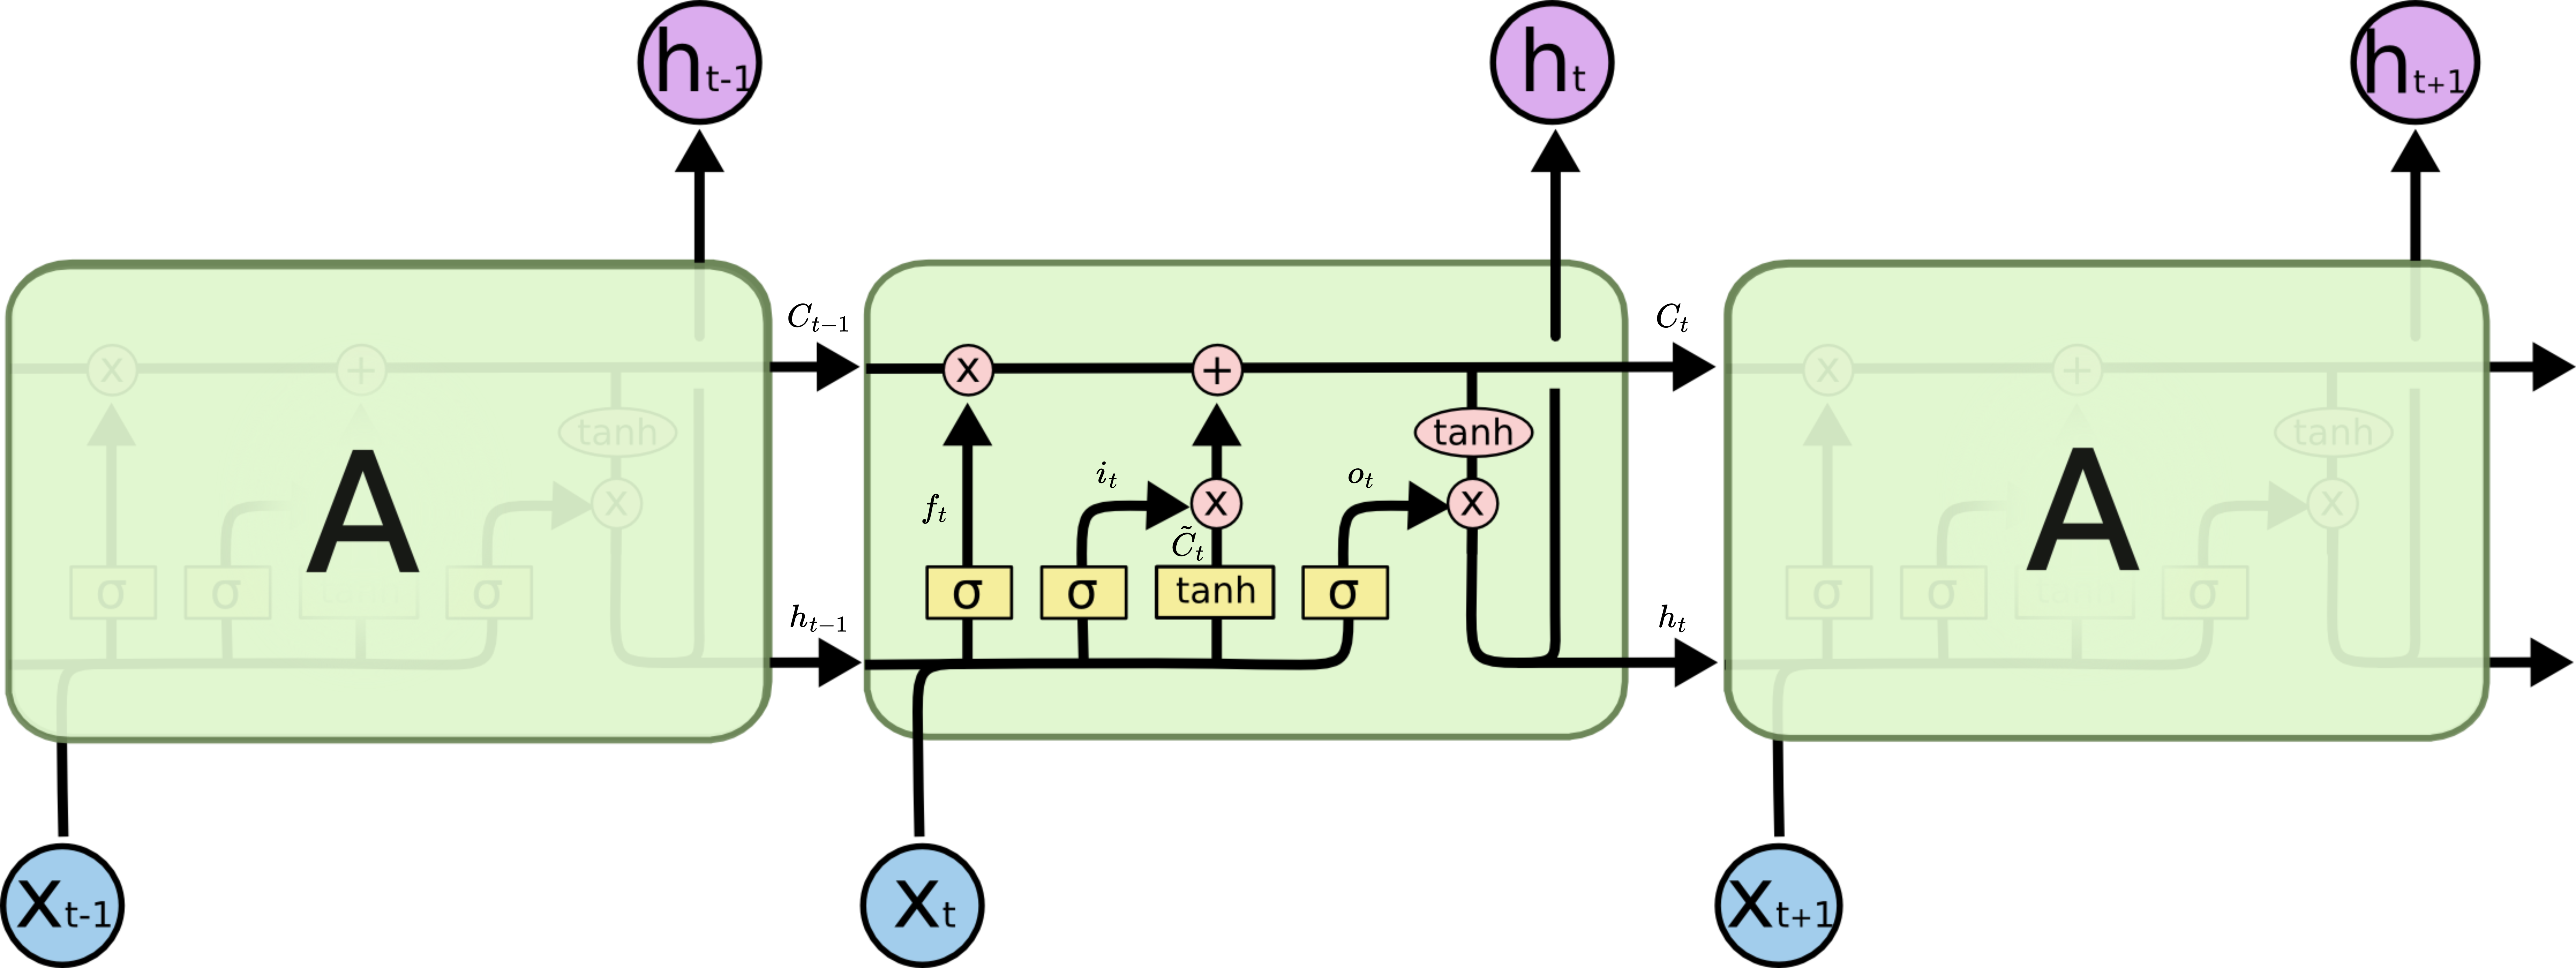
\includegraphics[width=0.9\textwidth]{LSTM Architecture.drawio.png}
  \caption{The repeating module of an LSTM network. Each yellow box represents a neural
    network layer with its activation function and the pink circles represent pointwise
    operations. The lines merging denote concatenation, while a line forking denotes its
    content being copied. The output is denoted by $h_t$. \cite{olahUnderstandingLSTM}}
  \label{fig:lstm}
\end{figure}

The architecture of an LSTM network is based on a repeating module containing four
interacting layers, as shown in \reffig{fig:lstm}. The central feature of LSTMs is the
cell state $C_t$, which runs straight down the entire chain with only minor linear
interactions. This allows information to flow unchanged along the cell state, making it
easy for the network to remember information over long time scales. The cell state is
controlled by structures called gates, which are made up of neural network layers and
pointwise operations. The gates enable the network to remember or forget information as
needed.


\subsubsection{Forget Gate}
\label{sec:3.0.0}

The first step in the operation of an LSTM is to decide which information from the cell
state to forget. This is done by a sigmoid layer which takes the previous hidden state
$h_{t-1}$ and the current input $x_t$ as input and outputs a number between $0$ and $1$
for each element in the cell state $C_{t-1}$. A value of $0$ indicates that the
corresponding element should be forgotten, while a value of $1$ indicates that it should
be retained. The network can then filter out unimportant information and focus on what
matters.
\begin{equation}
  f_t = \sigma(W_f \cdot [h_{t-1}, x_t] + b_f)
\end{equation}


\subsubsection{Input Gate}
\label{sec:3.0.1}

The next step is to decide what new information to store in the cell state. It has two
parts. First, a sigmoid layer decides which values to update. Next, a tanh layer creates a
vector of new candidate values $\tilde{C}_t$ that could be added to the state. The input
gate layer outputs a number between $0$ and $1$ for each element in the cell state,
indicating how much of the new candidate values should be added to the state. Thus, the
network can selectively update the cell state with new information.
\begin{align}
  i_t         & = \sigma(W_i \cdot [h_{t-1}, x_t] + b_i) \\
  \tilde{C}_t & = \tanh(W_C \cdot [h_{t-1}, x_t] + b_C)
\end{align}


\subsubsection{Update Cell State}
\label{sec:3.0.2}

The next step is to update the old cell state $C_{t-1}$ into the new cell state $C_t$.
First, the old state is multiplied by the forget gate $f_t$, forgetting the things that
were decided to forget earlier. Then, the new candidate values $\tilde{C}_t$ are added to
the state, scaled by how much the input gate decided to update each state value.
\begin{equation}
  C_t = f_t \cdot C_{t-1} + i_t \cdot \tilde{C}_t
\end{equation}


\subsubsection{Output Gate}
\label{sec:3.0.3}

Finally, the network needs to decide what to output. This output will be based on the cell
state, but will be a filtered version. First, a sigmoid layer decides which parts of the
cell state to output. Then the cell state is run through a tanh function to shift the
values between $-1$ and $1$, and multiplied by the output of the sigmoid gate. The result
is the output of the network at the current time step $h_t$, which can be used for further
processing or as the final output of the network.
\begin{align}
  o_t & = \sigma(W_o \cdot [h_{t-1}, x_t] + b_o) \\
  h_t & = o_t \cdot \tanh(C_t)
\end{align}


\subsection{Variants}
\label{sec:3.1}

% Variant: Peephole Connections
LSTMs have been the subject of extensive research, leading to the development of several
variants \cite{greffLSTMSearchSpace2017}. One popular variant, introduced by Gers and
Schmidhuber in 2000 \cite{gersRecurrentNetsTime2000}, adds peephole connections to the
LSTM architecture. These connections allow the cell to control the gates more precisely,
making it easier for the network to learn precise timing. In addition, the output
activation function is omitted, as there is no evidence that it is essential for solving
the problems on which LSTMs have been tested so far.

% Variant: Dynamic Cortex Memory
Another variant, called Dynamic Cortex Memory (DCM), was introduced by Otte et al. in 2014
\cite{otte2014dynamic}. DCM adds several new trainable connections to the LSTM model,
improving the error carousel and the internal interplay between gates. These connections
make direct signal transmission between the gates possible, resulting in faster
convergence than LSTM under the same training conditions. Furthermore, DCMs outperform
LSTMs in generalisation, as shown for several supervised problems, including precise value
storage, addition, and context-sensitive grammar learning.

% Variant: Gated Recurrent Unit

\begin{figure}[htbp]
  \centering
  \includegraphics[width=0.9\textwidth]{LSTM3-var-GRU.png}
  \caption{The structure of a Gated Recurrent Unit (GRU) network. \cite{olahUnderstandingLSTM}}
  \label{fig:gru}
\end{figure}
One of the best known variants of the LSTM architecture is the Gated Recurrent Unit (GRU),
which was proposed by Cho et al. in 2014 \cite{choLearningPhraseRepresentations2014}. The
GRU simplifies the LSTM architecture by removing the output gate and the cell state, and
combining the input and forget gates into a single update gate. This reduces the number of
parameters in the network and makes it easier to train. The internal structure of a GRU
network is shown in \reffig{fig:gru}. While the GRU has been shown to perform comparably
to the LSTM for many tasks, it has the advantage of being simpler and more efficient,
making it a popular choice for many applications \cite{Yang2020}.



\section{Neural Turing Machines}
\label{ch:4}

While LSTMs and their variants have proven effective for a wide range of tasks, they are
still limited in their ability to perform complex operations that require explicit memory
access. To address this limitation, Graves et al. introduced the Neural Turing Machine
(NTM) in 2014 \cite{gravesNeuralTuringMachines2014}. The NTM is augmented with an external
memory bank to combine the power of neural networks with the capability to store and
retrieve information. Unlike operations on a computer's memory, the NTM's operations are
designed to be fully differentiable and can be trained using backpropagation and
gradient-based optimisation algorithms.

The approach is inspired by the structure and operation of a Turing machine, which is a
theoretical model of a computer that can read from and write to an infinite tape of
memory. A computer program uses three basic mechanisms: elementary operations (such as
arithmetic), logical flow control (branching), and external memory that can be written to
and read from during computation \cite{von_neumann_first_1945}. In human cognition, the
process that most closely resembles algorithmic operation is known as working memory,
which is understood as the capacity for short-term storage of information and its
rule-based manipulation \cite{baddeley_memory_2009}.


\subsection{Architecture}
\label{sec:4.0}

\begin{figure}[htbp]
  \centering
  \includegraphics[width=0.7\textwidth]{NTM Structure.png}
  \caption{The architecture of a Neural Turing Machine.}
  \label{fig:ntm-structure}
\end{figure}

The architecture of an NTM, as shown in \reffig{fig:ntm-structure}, consists of two main
components: a controller and a memory bank. The controller is an LSTM, which is
responsible for processing the input data and interacting with the memory bank. The memory
bank for time step $t$ is a matrix $\textbf{M}_t$ of size $N \times M$, where $N$ is the
number of memory locations and $M$ is the size of each memory location. The memory bank
can be read from and written to by the controller. It interacts with the memory bank using
read heads and write heads, which are responsible for reading and writing information from
and to the memory bank. They use an attention mechanism to select the memory locations,
allowing the network to focus on specific parts of the memory.


\subsection{Addressing Mechanism}
\label{sec:4.1}

\begin{figure}[htbp]
  \centering
  \includegraphics[width=0.9\textwidth]{ntm_addr_4.png}
  \caption{Flow diagram of the addressing mechanism in a Neural Turing Machine.
    \cite{gravesNeuralTuringMachines2014}}
  \label{fig:ntm-addressing}
\end{figure}

The addressing mechanism of an NTM is responsible for selecting the memory locations to
read from and write to. It combines both content-based and location-based addressing and
consists of four main steps: content addressing, interpolation, convolutional shift and
sharpening, as shown in \reffig{fig:ntm-addressing}. The addressing mechanism is performed
at each time step, providing a dynamic and flexible way for the controller to interact
with the memory bank.


\subsubsection{Content Addressing}
\label{sec:4.1.0}

The first step of the addressing mechanism is content addressing, which selects memory
locations based on the content of the cells. It takes as input the current memory bank
$\textbf{M}_t$, the key vector $\textbf{k}_t$, and the key strength $\beta_t$. The key
vector is used to calculate the similarity between the key and each memory location using
the cosine similarity measure $K[\cdot, \cdot]$. The parameter $\beta_t$ amplifies the
precision of the attention weights, enforcing high sparsity in the weights.
\begin{equation}
  \textbf{w}_t^c = \text{softmax}(\beta_t K[\textbf{M}_t, \textbf{k}_t])
\end{equation}


\subsubsection{Interpolation}
\label{sec:4.1.1}

The next step is interpolation, which lets the network iteratively access subsequent
memory locations. It uses the previous attention weights $\textbf{w}_{t-1}$, the
content-based attention weights $\textbf{w}_t^c$, and the interpolation gate $g_t \in (0,
  1)$. For a value of $g_t = 0$ the previous weights are retained, while for a value of $g_t
  = 1$ the current weights are used. This enables the network to blend between them based on
the value of $g_t$.
\begin{equation}
  \textbf{w}_t^g = g_t \textbf{w}_t^c + (1 - g_t) \textbf{w}_{t-1}
\end{equation}


\subsubsection{Convolutional Shift}
\label{sec:4.1.2}

After interpolation, each head produces a shift weighting $\textbf{s}_t$ that is used as
the kernel for a convolutional shift operation. It convolves the new attention weights
with the kernel $\textbf{s}_t$, allowing the network to shift the attention if needed.
This is useful for accessing memory locations dynamically. All indices are modulo
$N$ to ensure that the shift operation is circular.
\begin{equation}
  \tilde{\textbf{w}}_t(i) \leftarrow \sum_{j=0}^{N-1} \textbf{w}_t^g(j) \textbf{s}_t(i-j)
\end{equation}


\subsubsection{Sharpening}
\label{sec:4.1.3}

The final step of the addressing mechanism is sharpening, which amplifies the focus of the
attention weights. It takes the convolved attention weights $\tilde{\textbf{w}}_t$ and the
sharpening parameter $\gamma_t \geq 1$ as input and applies a power function to the
weights, increasing large weights and decreasing small weights. The effect of sharpening
increases with higher values of $\gamma_t$.
\begin{equation}
  \textbf{w}_t(i) = \frac{\tilde{\textbf{w}}_t(i)^{\gamma_t}}{\sum_{j} \tilde{\textbf{w}}_t(j)^{\gamma_t}}
\end{equation}


\subsection{Comparison with LSTMs}
\label{sec:4.2}

To compare the performance of the NTM with LSTMs, Graves et al. conducted a series of
experiments on a set of simple algorithmic tasks, such as copying and sorting data
sequences. The aim was to show that the NTM is able to solve the problems by learning
compact internal programs. For example, the researchers tested whether a network trained
to copy sequences up to 20 in length could copy a sequence up to 120 in length without
further training. The results of the experiments showed that the NTM was able to learn
much faster than LSTMs and converged to a lower cost. In addition, the NTM was able to
generalise well beyond the range of the training data, while the LSTM degraded rapidly
beyond length 20. This suggests that the NTM, unlike the LSTM, had learned some form of
copying algorithm. The researchers also examined the interaction between the controller
and memory, and concluded that the NTM had learned how to create and iterate through
arrays. The focus-sharpening mechanism was also found to be essential, as without it the
weightings would lose precision over time.


\section{Conclusion}
\label{ch:5}

In this paper we have explored the architecture and operation of Recurrent Neural
Networks, Long Short-Term Memory networks and Neural Turing Machines, focusing on their
ability to store and retrieve information over long time scales. We looked at their
internal structure, the back-propagation algorithm used to train them, the problem of
long-term dependencies in standard RNNs, and introduced LSTMs as a solution to this
problem. We also discussed the architecture of LSTMs and their variants and introduced the
Neural Turing Machine built on top of the LSTM architecture. The results of experiments
comparing the performance of LSTMs and NTMs on a set of simple algorithmic tasks were
presented, showing that the NTM was able to learn these specific tasks much faster with
higher accuracy than LSTMs. Overall, the field of RNNs and their variants is a rapidly
developing area of research, and we expect to see many more exciting developments in the
future.



\newpage
\nocite{}
\bibliographystyle{plain}
\bibliography{report}

\end{document}

